% !TeX spellcheck = en_GB
% !TEX root = ../thesis.tex

\chapter{Symmetry analysis} \label{ch:symmetry}

\begin{chapterabstract}
		
	As discussed in Chapter \ref{ch:intro}, it is possible to create topological modes by opening a suitable gap in $k$-space, which may be achieved by breaking the symmetry of a metamaterial pattern. In this Chapter, we take a step back and analyse the concept of symmetry in a very general manner. Our aim is to determine the constraints symmetries impose on the band structure, and its fate when they are broken. As a preliminary, we describe the concept of excitations in linear media. We then introduce in Sec.~\ref{sec:symm_groups} a self-contained framework adapted from the theory of space groups, which serves to find band structure degeneracies, followed by a perturbative approach to describe symmetry breaking in Sec.~\ref{sec:symm_perts}. Finally, we apply the introduced concepts on sixfold and fourfold symmetric lattices in Secs.~\ref{sec:symm_sixfold} and \ref{sec:symm_fourfold}, discussing the various effects which may be induced in engineered metamaterials. 	
	%
	\tcblower
	%
	Parts of this Chapter are taken from the Supplemental Material of Ref.~\cite{Kosata_2021}.
\end{chapterabstract}

In general, an excitation $\psi(\vb{r} ,t)$ in a linear medium is governed by a linear equation of motion
\begin{equation} \label{eq:symm_eom_gen}
\mathcal{L} \psi(\vb{r}, t) =  0 \,,
\end{equation}
where $\mathcal{L}$ is a linear operator, typically consisting of partial derivatives with respect to time and space.
Such problems are ubiquitous in many fields of classical and quantum physics. For example, Maxwell's equation describing the out-of-plane electric field $\mathcal{E}(\vb{r}, t)$ in a 2D medium of relative permittivity $\epsilon_r(\vb{r})$,
\begin{equation} \label{eq:symm_maxwell}
\left[ \frac{1}{\epsilon_r(\vb{r})} \nabla \cross \nabla - \frac{1}{c^2}\frac{\partial^2}{\partial t^2} \right] \mathcal{E}(\vb{r}, t) = 0 \,,
\end{equation}
and the Schr\"{o}dinger equation for the quantum-mechanical wavefunction $\psi(\vb{r}, t)$ subject to a Hamiltonian $H(\vb{r})$,
\begin{equation} \label{eq:symm_se}
\left[H(\vb{r}) - i \hbar \frac{\partial}{\partial t} \right] \psi(\vb{r}, t) = 0 \,.
\end{equation}
Similar equations apply in countless other domains, including acoustics, elasticity, polaritonics, electronics and hydrodynamics.

The form of Eqs.~\eqref{eq:symm_maxwell} and \eqref{eq:symm_se} suggests a separation of the temporal and spatial variables, as well as harmonic time-dependence,
%
\begin{equation} \label{eq:symm_sol_gen}
\psi(\vb{r}, t) = \e^{-i \omega t} \phi(\vb{r}) + \text{c.c.} 
\end{equation}
%
This allows us to drop the explicit time-dependence to get,
\begin{equation} \label{eq:symm_linproblem}
L \phi(\vb{r}) = E(\omega) \phi(\vb{r})\,,
\end{equation}
where $L$ is a linear operator in real space. The interpretation of the eigenvalue $E(\omega)$ depends on the physical context. Often, it expresses the energy of the excitation, in which case $L$ is the Hamiltonian. In the rest of this Section, we shall be analysing Eq.~\eqref{eq:symm_linproblem}.

As we focus on periodic structures, we express the spatial part as a Bloch function\footnote{In the presence of discrete time-translation symmetry, the time dependence may also be expressed as a Bloch function. The study of such solutions is called \textit{Floquet theory}.}. Assuming a lattice vector $\vb{a}$, we may choose a vector $\vb{k}$ to construct a solution of the form
\begin{equation} \label{eq:symm_sol_gen_space}
\phi_{\vb{k}}(\vb{r}) = u_{\vb{k}}(\vb{r}) \e^{i \vb{k} \vdot \vb{r}} \,, \qquad u_{\vb{k}}(\vb{r} + \vb{a}) = u_{\vb{k}}(\vb{r}) \,,
\end{equation}
The functional dependence of $E(\omega)$ on $\vb{k}$ is then known as \textit{dispersion}.

We may now impose symmetry constraints on $\phi(\vb{r})$ and the resulting eigenvalue spectrum. Before plunging into a formal presentation of the necessary concepts, we attempt an informal explanation to guide our efforts in this Chapter. 

\subsubsection{Informal summary} 

The solution $\phi_{\vb{k}}(\vb{r})$ must obey the symmetries of the underlying medium, i.e., of the governing equations such as \eqref{eq:symm_maxwell} and \eqref{eq:symm_se}. This means that for every spatial transformation $g$ which leaves the medium self-coincident, $\phi_{\vb{k}}(g \vb{r})$ must also be a valid solution with the same eigenvalue as $\phi_{\vb{k}}(\vb{r})$. The transformation $g$ affects both the underlying unit cell solution $u_{\vb{k}}(\vb{r})$ and the $\vb{k}$ label,
\begin{equation}
u_{\vb{k}}(\vb{r}) \e^{i \vb{k} \vdot \vb{r}}\quad \xrightarrow{\mathmakebox[1.5em]{g}} \quad u_{\vb{k}}(g \vb{r}) \e^{i \vb{k} \vdot g \vb{r}} = u_{\vb{k}}(g \vb{r}) \e^{i g^{-1} \vb{k} \vdot \vb{r}} \,.
\end{equation}
When this mapping results in a distinct solution, a degeneracy occurs. Degenerate solutions may have the same or different $\vb{k}$ labels. The set of degenerate solutions mapped into each other form a \textit{basis for an irreducible representation} -- we find these in Sec.~\ref{sec:symm_groups}.
%We explore the degeneracy by finding a \textit{basis} -- a set of functions $u_{\vb{k}}(\vb{r}) \e^{i \vb{k} \vdot \vb{r}}$ closed under the action of all symmetry operations.

With an explicit basis at hand, we may represent each symmetry operation by a matrix -- its \textit{representation matrix}, which must commute with our linear operator $L$. Perturbing the structure then removes one of these symmetry requirements, allowing for the degeneracy to split in a way that preserves the remaining symmetries. The degeneracy will typically only hold at a specific point $\vb{k}$ and not in its vicinity, giving rise to Dirac cones.

To get any further, we must now introduce the much more precise language of group and representation theory.

\section{Band structures from space group theory} \label{sec:symm_groups}

In this Section, we introduce the necessary group-theoretical concepts and derive the symmetry-imposed band structure degeneracies. For both subsections, we give a terse technical overview followed by an accessible example. The formalism follows the exposition of Ref.~\cite{Bradley_2009}, a useful introduction can also be found in Ref.~\cite{Cano_2018}. 

\subsection{Glossary}

\textit{Group: } A set $\mathcal{G}$ of elements along with a binary operation which combines any two to form another group element. This must fulfil the three group axioms, (i) the operation is associative, (ii) there exists an identity element $e$ such that $g e = g$ for all $g \in \mathcal{G}$, (iii) the group contains an inverse of each element, i.e., for each $g \in \mathcal{G}$, there is a $h \in \mathcal{G}$ such that $g h = e$.  

\textit{Point group: } A group of symmetry operations that have a fixed point in common. Here we shall use $n$-fold rotations ($C_n$), reflections about a mirror plane ($\sigma_x, \, \sigma_y$) and inversion ($I$).

\textit{Generator:} A set of operations $g \in G$ whose combinations generate every element of $\mathcal{G}$. 

\textit{Symmorphic space group:} The group $\mathcal{G}$ generated by a set composed of point group operations and real space translations is called symmorphic\footnote{Equivalently, a symmorphic group has no glide planes or screw axes.}.

\textit{Isogonal group:} The point group operations of a symmorphic space group $\mathcal{G}$ form its isogonal group $\mathcal{F} \subset \mathcal{G}$. For symmorphic space groups, we may always choose a unit cell with the symmetries of the isogonal group.

\textit{Equivalent $k$-points:} Two points in $k$-space are equivalent if they differ by a combination of reciprocal lattice vectors.

\textit{Little co-group:} For a space group $\mathcal{G}$, the point group operations which take a $k$-space vector $\vb{k}$ into an equivalent point form the little co-group of $\vb{k}$, denoted ${{\overline{\mathcal{G}}}_{\vb{k}}} \subset \mathcal{F}$.

\textit{Star:} The set of inequivalent $k$-points generated from $\vb{k}$ by all operations of a group $\mathcal{G}$ is called the star of $\vb{k}$.

\textit{Representation:} The representation $\rho$ of a group $\mathcal{G}$ is a homomorphism of $\mathcal{G}$ onto a group $\mathcal{T}$ of non-singular linear operators acting in a finite-dimensional vector space $V$. If $V$ has no subspace invariant under the operations of $\mathcal{T}$ other than $V$ itself, then $\rho$ is an \textit{irreducible representation (irrep)}.

\textit{Basis for an irrep:} A set of functions $B$ that spans the domain $V$ of an irrep $\rho$ is a basis of $\rho$. Each basis belongs to one irrep only.

\textit{Representation matrix:} Having chosen a basis $B$, every symmetry element $g \in \mathcal{G}$ is mapped by $\rho$ onto a matrix $\rho(g) \in \mathcal{T}$. This is the representation matrix of $g$ in the basis $B$.

\subsubsection{Example: the \textit{p6m} space group}

To illustrate the above terminology, we describe the space group \textit{p6m} exemplified by graphene, shown in Fig.~\ref{fig:symm_graphene}(I). Its symmetry elements are generated by three operations: a sixfold rotation around the unit cell centre ($C_6$), spatial inversion ($I$) and a lattice vector translation ($\vb{a}$)\footnote{The choice of the unit cell is, strictly speaking, arbitrary, but choosing the highest-symmetry cell is very convenient. For example, suppose we chose a unit cell centred on one of the atomic sites -- such a cell is related to the highest-symmetry cell by a translation, $\vb{b}$. The sixfold rotation $C_6$ would therefore appear as a composite operation $\vb{b}^{-1} C_6 \vb{b}$.}. The space group of this structure is therefore \textit{p6m}\footnote{More precisely, the symmetry operations form a group which is isomorphic to \textit{p6m}.} and the isogonal group is $C_{6v}$. Symmetry analysis for the different $k$-points, marked in Fig.~\ref{fig:symm_graphene}(III), follows.

\begin{figure} [h!]
	\centering
	\includesvg{figures/symmetries/graphene.svg}
	\caption{(I) The unit cell of graphene, with atoms shown as red spheres and the lattice vector $\vb{a}$ marked. (II) Its equivalent continuous model -- a honeycomb lattice of incisions (grey) in a linear medium (blue). (III) The corresponding Brillouin zone.}
	\label{fig:symm_graphene}
\end{figure} 

$\boldsymbol{\Gamma}$: The point $\boldsymbol{\Gamma} = (0,0)$ is invariant under all point group operations. Hence, its little co-group is the same as the isogonal group, $C_{6v}$, which implies that the star $S = \{ \boldsymbol{\Gamma} \}$.

$\boldsymbol{M}$: The point $\boldsymbol{M} = \frac{2\pi}{3 \abs{\vb{a}}} \left(1,\,0 \right)$ is taken into an equivalent $k$-point, $-\boldsymbol{M}$, by spatial inversion and a $C_2$ rotation, giving a little co-group $C_{2v}$. A $C_6$ rotation brings it into an inequivalent point $\boldsymbol{M}'$, so that the star is $S = \{ \boldsymbol{M}, \boldsymbol{M}' \}$. 

$\boldsymbol{K}$: The point $\boldsymbol{K} =  \frac{2\pi}{3 \abs{\vb{a}}} \left(1,\, 1/\sqrt{3} \right)$ is taken into an equivalent $k$-point by a $C_3$ rotation and a vertical mirror plane, giving a little co-group $C_{3v}$. The star is again generated by a $C_6$ rotation: $S = \{\boldsymbol{K}, \boldsymbol{K}' \}$. 

$\boldsymbol{P}$: This is a general point with no special symmetries. Its little co-group is $C_1$ and the star is six-membered, $S = \{ \boldsymbol{P}, R_6 \boldsymbol{P}, \, \ldots ,\, R_6^5 \boldsymbol{P} \}$, where $R_6$ is a $2\pi/6$ rotation matrix. 


\subsection{Constructing an irrep and its basis} \label{sec:symm_irrep_cons}
We mentioned that the irreps of a space group determine degeneracies in the Brillouin zone. As it turns out, however, it is simpler to construct an explicit basis straight away rather than search for irreps. It also has the added benefit of providing us with representation matrices for the symmetry operations, which will be very useful later. 

We now describe a step-by-step procedure for constructing a basis. We consider a space group $\mathcal{G}$ with the isogonal group $\mathcal{F}$, and seek a basis $B = \{\phi_j(\vb{r}) \}$ for a yet-unknown irrep $\rho$. We look for a set of Bloch functions of the type
\begin{equation} \label{seq:blochfunc}
\phi_j(\vb{r}) = u_j(\vb{r}) \e^{i \vb{k} \vdot \vb{r}}\,,
\end{equation}
where $\vb{k}$ is a $k$-space vector, and $u_j(\vb{r})$ is invariant under lattice translations. In such a basis, the representation matrix of translation by a unit cell, $\rho(\vb{a})$, is diagonal, as it only introduces phase shifts. Choosing a vector $\vb{k}$, we now proceed in three steps. For brevity, we omit brackets.

(i)~Determine the little co-group ${\overline{\mathcal{G}}}_{\vb{k}}$. For every $g \in {\overline{\mathcal{G}}}_{\vb{k}}$, we have $g \left(u_j\, \e^{i \vb{k} \vdot \vb{r}}\right) = \e^{i \vb{k} \vdot \vb{r}} \,g u_j$ by definition, up to a periodic function which can be absorbed into the definition of $u_j$. To be closed under ${\overline{\mathcal{G}}}_{\vb{k}}$, the set $\{u_j\}$ must therefore form a basis for its representation. Let us then choose a $b$-dimensional irrep $\rho_{\vb{k}}$ of $\overline{\mathcal{G}}_{\vb{k}}$, and a basis $B_{\rho_{\vb{k}}}$ of $\rho_{\vb{k}}$ such that every $u_j \in B_{\rho_{\vb{k}}}$ is invariant under lattice translations. Each $u_j \in B_{\rho_{\vb{k}}}$ can be used to define $u_j\, \e^{i\vb{k}\vdot\boldsymbol{r}} \in B$. We have thus constructed $b$ basis functions of the irrep $\rho$.

(ii)~Take an element $h \in \mathcal{F}$ that is not in ${\overline{\mathcal{G}}}_{\vb{k}}$. As such, $h$ maps a Bloch function labelled by $\vb{k}$ into another member of its star, $h \left(\e^{i \vb{k}\vdot\vb{r}}\right) = \e^{i \vb{k}'\vdot\vb{r}}$. The transformed basis $h \left( B_{\rho_{\vb{k}}}\right)$ is still a basis of $\rho_{\vb{k}}$, although generally ${B_{\rho_{\vb{k}}}} \neq h \left( B_{\rho_{\vb{k}}}\right)$. From each function $h  \left(u_j\right) \in h \left( {B_{\rho_{\vb{k}}}}\right)$, we again generate a $h  \left(u_j\right)\, \e^{i \vb{k}'\vdot\vb{r}} \in B$.

(iii)~Repeat step (ii) for each inequivalent $\vb{k}$ generated by $h$. 

For a $\vb{k}$ with a $q$-membered star and a $b$-dimensional irrep of ${\overline{\mathcal{G}}}_{\vb{k}}$, we have thus generated a $(qb)$-dimensional basis for an irrep $\rho$ of $\mathcal{G}$. In the band diagram, this appears as $q$ points, each $b$-fold degenerate. The representation matrix of each operation in $\mathcal{G}$ is found explicitly by its action in the basis $B$.


\subsubsection{Time-reversal symmetry}

Spatial symmetries are not the only constraint imposed on our system. Unless otherwise specified, a static material possesses time-reversal (TR) symmetry, which has implications on its band structure. Referring to our ansatz \eqref{eq:symm_sol_gen} reveals that imposing a transformation $t \rightarrow -t$ on the solution of our linear problem gives
\begin{equation}
\begin{gathered}
\psi(\vb{r}, t) = \e^{i \left( \vb{k} \vdot \vb{r} - \omega t \right)} u_{\vb{k}}(\vb{r}) + \e^{-i \left( \vb{k} \vdot \vb{r} - \omega t \right)} u_{\vb{k}}(\vb{r})^* \\
\xrightarrow{\text{TR}} \e^{-i \left( -\vb{k} \vdot \vb{r} - \omega t \right)} u_{\vb{k}}(\vb{r}) + \e^{i \left( -\vb{k} \vdot \vb{r} - \omega t \right)} u_{\vb{k}}(\vb{r})^* \,,
\end{gathered}
\end{equation}
which is equivalent to taking
\begin{equation} \label{eq:symm_trs}
u_{\vb{k}}(\vb{r}) \rightarrow u_{\vb{k}}(\vb{r})^* \,, \quad \vb{k} \rightarrow -\vb{k} \,,
\end{equation}
which must again yield a valid solution. Eq.~\eqref{eq:symm_trs} will allow us to impose (or break) TR symmetry despite not dealing explicitly with the time dimension. 

\subsubsection{Example: \textit{p6m} continued}

We now construct a basis for one of the irreducible representations of \textit{p6m}. Referring to our discussion above, the expected degeneracies depend on the size of the star, and the irreps of the little co-group\footnote{The irreducible representations and their bases are tabulated for common point groups~\cite{Bradley_2009}.} of each respective point in $k$-space, as summarised in Table \ref{table:symm_p6m_degs}.
\begin{table} [h!]
 		\centering
 		\caption{Properties of different $k$-points of the \textit{p6m} space group. }
		\label{table:symm_p6m_degs}
 	\begin{tabular}{ c c c c c }
 		$k$ point & $\boldsymbol{\Gamma}$ & $\boldsymbol{M}$ & $\boldsymbol{K}$ & $\boldsymbol{P}$  \\ \hline
 		little co-group irrep dimensions & 1, 2 & 1 & 1, 2 & 1 \\
 		star members & 1 & 2 & 2 & 6 \\
 		solution degeneracy & 1, 2 & 2 & 2, 4 & 6 \\
 	\end{tabular}
\end{table}

Somewhat counter-intuitively, it is the low-symmetry point $\boldsymbol{P}$ which shows the highest solution degeneracy. However, this degeneracy is hardly useful for mimicking the physics of Dirac cones. To do that, we must use one of the high-symmetry points. As discussed in Chapter~\ref{ch:intro}, a TR-symmetric emulation of the quantum spin and valley Hall effects requires a 4-band model. For this reason, we will now focus on the $\boldsymbol{K}$ point. Note however that the degeneracies at $\boldsymbol{M}$ and $\boldsymbol{\Gamma}$ are also interesting -- these may emulate the Hall effect, which only needs a 2-band model. 

The star of $\boldsymbol{K}$ has two members; seeking a fourfold degeneracy, we focus on the 2-dimensional irrep of $C_{3v}$. A possible basis for this irrep is $(x,y)$;  we therefore define functions $(u_x(\vb{r}), u_y(\vb{r}))$, which transform as $(x,y)$ under point group operations, but are invariant under lattice translations. Applying steps (i) and (ii) with $h = C_6$ gives four basis functions of \textit{p6m}. Omitting the brackets, these are
%
\begin{equation} \label{seq:basis}
\{ u_x \e^{i \boldsymbol{K} \vdot \vb{r}}, u_y \e^{i \boldsymbol{K} \vdot \vb{r}}, u_x \e^{i \boldsymbol{K'} \vdot \vb{r}}, u_y \e^{i \boldsymbol{K'} \vdot \vb{r}} \} \,.
\end{equation}
%
Let us now find the representation matrices of the symmetry elements. The translation $\vb{a}$ is diagonal, containing phase shifts due to the $\boldsymbol{K}/\boldsymbol{K'}$ labels,
%
\begin{equation}
\rho(\vb{a}) = \text{diag}\{ \e^{4 \pi i /3}, \e^{2 \pi i /3}  \} \otimes \mathbb{1}_2\,.
\end{equation}
%
The mirror plane $\sigma_x \notin \overline{\mathcal{G}}_{\boldsymbol{K}}$ maps $(u_x,u_y) \rightarrow (u_x, -u_y)$ and $(\boldsymbol{K}, \boldsymbol{K}') \rightarrow (\boldsymbol{K}', \boldsymbol{K})$, and thus gives
%
\begin{equation}
\rho(\sigma_x) = \tau_1 \otimes \tau_3,
\end{equation}
%
where $\tau$ are the Pauli matrices.
Finally the rotation $C_6 \notin \overline{\mathcal{G}}_{\boldsymbol{K}}$ maps $(u_x, u_y) \rightarrow R_6 (u_x,u_y)$, where $R_6$ is the $2\pi/6$ rotation matrix, and $(\boldsymbol{K}, \boldsymbol{K}') \rightarrow (\boldsymbol{K}', \boldsymbol{K})$, giving in our basis choice
\begin{equation}
\rho(C_6) = \tau_1 \otimes R_6\,.
\end{equation}
Note that while this proves the existence of such an irrep, the particular choice of basis is unimportant. Numerical solutions of a specific problem need not immediately resemble the form constructed in Eq.~\eqref{seq:basis}. The basis is chosen such that each $\rho(g)$ is a direct product of a $2 \times 2$ matrix acting on the two valley degrees of freedom with another $2 \times 2$ matrix acting on the two degenerate bands within each valley.

Finally, we express the TR operator in this basis according to the prescription shown in Sec.~\ref{sec:symm_irrep_cons},
\begin{equation}
\rho(\mathcal{T}) = (\tau_1 \otimes \mathbb{1}_2) \mathcal{K}
\end{equation}
where $\mathcal{K}$ is the complex conjugation operator. It is reassuring to notice that $\rho(\mathcal{T})$ commutes with all three of the spatial representation matrices. 

\section{Perturbation effects} \label{sec:symm_perts}

In general, for a continuous medium, the number of solutions $\phi(\vb{r})$ of the linear problem \eqref{eq:symm_linproblem} is infinite. In the previous Section, we formulated symmetry requirements that allowed us to group the solutions into degenerate sets, identifying each with an irrep of the underlying space group. 

Here, we make a conceptual leap and focus exclusively on a single set of degenerate solutions. It is within this restricted subspace that topological physics in metamaterials is usually realised. Such an approach is justified where the solutions lie in a bandgap, in which case no other solutions with similar eigenvalues are available for mixing. Where this is not the case (i.e., if accidental degeneracies are present), interactions of different solution sets must be considered~\cite{Benalcazar_2020, Cerjan_2020}.

We apply the concepts introduced in Sec.~\ref{sec:symm_groups} to obtain symmetry-allowed perturbative terms in our linear problem \eqref{eq:symm_linproblem}\footnote{Although adapted for our purposes, much of this material is covered in Refs.~\cite{Saba_2017, Saba_2020}.}.
Having chosen a basis where the solution appears as a vector $\vb{v}$, we have the equation
\begin{equation} \label{seq:eigenproblem}
M(\boldsymbol{\lambda})  \vb{v} = E(\boldsymbol{\lambda}) \vb{v} \,,
\end{equation}
where $M$ is a matrix (often, the Hamiltonian, in which case $E$ describes energy), and $\boldsymbol{\lambda}$ is a vector parametrising the perturbation.
\\

\subsubsection{Zeroth order} 

Suppose that the unperturbed operator $M(0)$ has a set of symmetries forming the space group $\mathcal{G}$. Take a set $V$ of vectors that correspond to a single eigenvalue $E(0)$.  If there are no accidental degeneracies, $V$ constitutes a basis for an irreducible representation of $\mathcal{G}$, thus uniquely defining the set of representation matrices $\rho(g)$. Correspondingly, for every $\vb{v} \in \text{span}(V)$ and $g \in \mathcal{G}$, we obtain a $\rho(g) \vb{v} \in \text{span}(V)$, such that
\begin{equation}
\begin{gathered}
M(0)\vb{v} = E(0) \vb{v} \quad \implies \quad M(0) \rho(g) \vb{v} = E(0) \rho(g) \vb{v} \\
\implies \quad \rho(g)^{-1} M(0) \rho(g) \vb{v} =  M(0) \vb{v} \,,
\end{gathered}
\end{equation}
Since $\vb{v}$ is arbitrary, we arrive at the kernel equation
\begin{equation} \label{seq:zeroconstraint}
M(0) = \rho(g)^{-1} M(0) \rho(g)\,,
\end{equation}
which, by construction, is satisfied only if $M(0) \propto \mathbb{1}$. In this case, the degeneracy is said to be \textit{symmetry-protected}, as any permissible perturbation must change all four eigenvalues simultaneously.
\\

\subsubsection{First order} 

We now perturb with a real parameter $\boldsymbol{\lambda}$ to the first order. Keeping the same basis. Eq.~\eqref{seq:eigenproblem} now reads
\begin{equation} \label{seq:perteq}
\left[\boldsymbol{\lambda} \vdot \boldsymbol{M}_{1}(\boldsymbol{\lambda})\right] \vb{v} = E_1(\boldsymbol{\lambda}) \vb{v}\,,
\end{equation}
where we defined a tensor $\boldsymbol{M}_{1}(\boldsymbol{\lambda})$ such that $\left[M_1(\boldsymbol{\lambda})\right]_j = \partial_{\lambda_j} M(\boldsymbol{\lambda} )$ are Hermitian matrices, and a scalar $E_{1}(\boldsymbol{\lambda}) = \boldsymbol{\lambda} \vdot \boldsymbol{\nabla_\lambda} E(\boldsymbol{\lambda} )$. 
For each $g \in \mathcal{G}$, transforming both sides and asserting the invariance of $E_1(\boldsymbol{\lambda})$ gives a condition analogous to Eq.~\eqref{seq:zeroconstraint}, with one important difference: the operator $\boldsymbol{\nabla}_{\boldsymbol{\lambda}}$ may itself transform non-trivially under the symmetry operations,
\begin{equation}
\boldsymbol{\nabla}_{\boldsymbol{\lambda}} \xrightarrow[]{g} R(g)   \boldsymbol{\nabla}_{\boldsymbol{\lambda}}\,,
\end{equation}
generating the condition
\begin{equation} \label{seq:condition}
\left[M_1(\boldsymbol{\lambda}) \right]_j =  \rho(g)^{-1} R(g)_{ij} \left[M_1(\boldsymbol{\lambda} )\right]_i \rho(g) \, .
\end{equation}
A symmetry-allowed perturbation term $\left[M_1(\boldsymbol{\lambda}) \right]_j$ must satisfy Eq.~\eqref{seq:condition} for each $g$ in the generating set of $\mathcal{G}$. This means that, having found the representation matrices $\rho(g)$ in Sec.~\ref{sec:symm_groups}, we now wish to solve the linear system \eqref{seq:condition}. To do this, we must now find the transformations $R(g)$ of the possible perturbations. 

\subsection{Structural and magnetic perturbations} \label{sec:symm_eng} 

If the spatial structure itself is altered, see Fig.~\ref{fig:symm_pert_types}(b), the perturbed system will generally belong to some space group $\mathcal{G'} \subset \mathcal{G}$. Only the elements $g' \in \mathcal{G'}$ now bring the lattice into self-coincidence, i.e., $R(g') = 1$, while $R(h) = 0$ for  $h \notin \mathcal{G'}$. We also have $R(\mathcal{T}) = 1$, meaning the resulting perturbation must commute with the TR representation matrix.
%
\begin{figure} [h!]
	\centering
	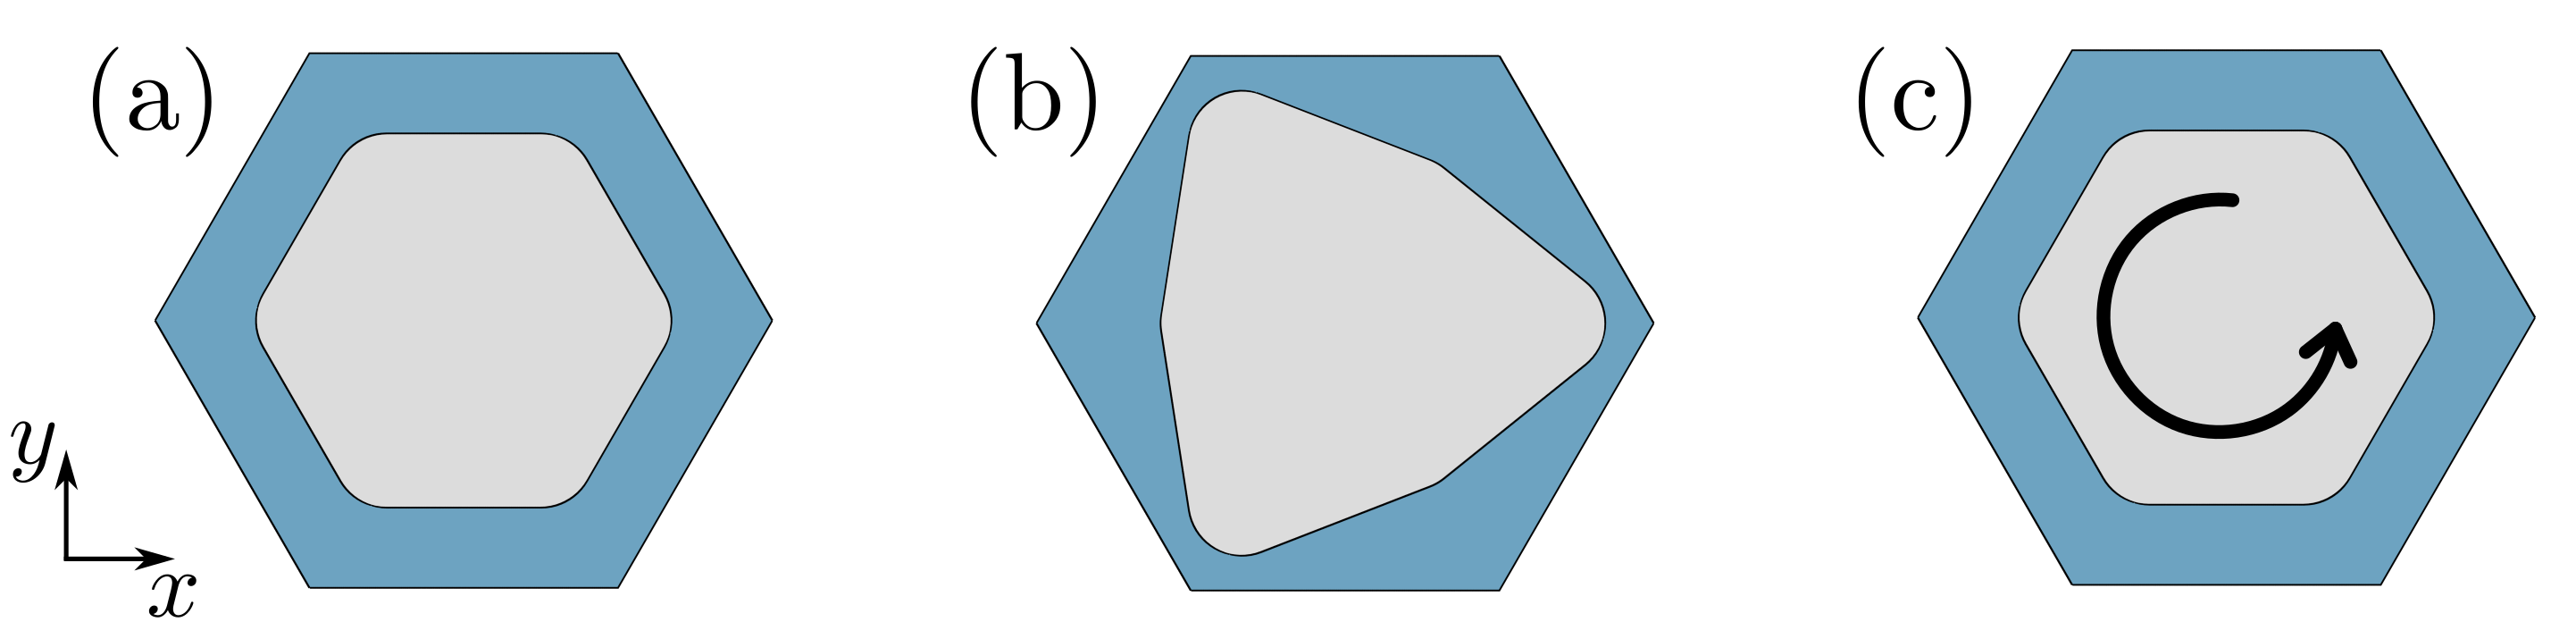
\includegraphics{figures/symmetries/pert_types.png}
	\caption{The two types of engineered perturbations. (a) An unperturbed unit cell belonging to the \textit{p6m} group, with symmetry elements $\{ C_6, \sigma_x, \vb{a}\}$. (b) A structural perturbation preserving $\{ C_3, \sigma_x, \vb{a}\}$, all with $R(g) = 1$. (c) A perturbing vector potential, corresponding to a magnetic field through the $z$-axis. This preserves all symmetry elements, with $R(C_6) = R(\vb{a}) = 1$ and $R(\sigma_x) = -1$.}
	\label{fig:symm_pert_types}
\end{figure}

A perturbation may also break TR symmetry, see Fig.~\ref{fig:symm_pert_types}(c). In this case, the symmetries are not necessarily lifted, but the perturbation may transform non-trivially under some symmetry elements. In the displayed example, the perturbation is inverted on applying $\sigma_x$, hence $R(\sigma_x) = -1$. Similarly, $R(\mathcal{T}) = -1$. 

While a ubiquitous way to create topological bandgaps, some engineered perturbations actually leave the degenerate solutions intact or merely shift them around in $k$-space. We elaborate on this point in Sec.~\ref{sec:symm_sixfold}. 

\subsection{Quasimomentum k} \label{sec:symm_kpert}

To find the behaviour of our solution away from the high-symmetry points in $k$-space, we consider a perturbation with $\boldsymbol{\lambda} = (\delta k_x, \delta k_y) = \vb{k} - \boldsymbol{K}$. The operator $\boldsymbol{\nabla}_{\vb{k}}$ transforms similarly to the vector $(x, y)$, for which the $2 \cross 2$ matrices $R(g)$ are readily found. The resulting perturbation is linearly proportional to $\vb{k}$, i.e., it describes linear dispersion. In some cases~\cite{Denner_2020}, this contribution vanishes, necessitating perturbations of higher order in $ \vb{k}$. Depending on the space group, symmetry-adapted basis vectors such as $(\delta k_x^2- \delta k_y^2, \delta k_x \delta k_y)$ are then a convenient basis choice. Note that this approach is essentially equivalent to that of $\vb{k} \vdot \vb{p}$ theory.

Equipped with the necessary framework, we now proceed to describe the various possible perturbations of six and fourfold symmetric lattices and their effects.

\section{Sixfold symmetry} \label{sec:symm_sixfold}
Here we shall again focus on the high-symmetry point $\boldsymbol{K}$ and the breaking of its fourfold solution degeneracy found in Table~\ref{table:symm_p6m_degs}.
We have already obtained the necessary representation matrices in the Example in Section \ref{sec:symm_groups},
\begin{equation} \label{eq:symm_six_rhos}
\begin{gathered}
\rho(C_6) = \tau_1 \otimes R_6 \, , \quad  \rho(\sigma_x) = \tau_1 \otimes \tau_3 \, , \\
\rho(\vb{a}) = \text{diag}\{ \e^{4 \pi i /3}, \e^{2 \pi i / 3} \} \otimes \mathbb{1}_2 \, , \quad \rho(\mathcal{T}) = (\tau_1 \otimes \mathbb{1}_2) \mathcal{K} \,.
\end{gathered}
\end{equation}
First, let us consider the perturbations associated with moving the quasimomentum $\vb{k}$ away from the high-symmetry points. Proceeding as outlined in Sec.~\ref{sec:symm_kpert}, we look for two $4 \cross 4$ matrices constrained by the condition \eqref{seq:condition}. This is a linear problem in 32 variables, which we solve in Wolfram Mathematica~\cite{Mathematica}, obtaining the allowed perturbation terms (notice that both anticommute with time reversal, $\rho(\mathcal{T})$)\textit{}
\begin{equation}
\delta k_x \left(\tau_3 \otimes \tau_1 \right) \equiv \delta k_x \gamma_x \,, \quad \delta  k_y \left(\tau_3 \otimes \tau_3 \right) \equiv \delta  k_y \gamma_y \,.
\end{equation} 
%
We therefore have an equation for the eigenvalues of our problem
%
\begin{equation} \label{eq:symm_ham}
\left[ \delta k_x \gamma_x + \delta k_y \gamma_y + M_1 \right] \vb{v} = (E-E_0) \,\vb{v} \,,
\end{equation}
where $E_0$ is the unperturbed eigenvalue and $M_1$ is given by structural and/or magnetic perturbations, cf. Sec.~\ref{sec:symm_eng}. We show examples of these in Table \ref{table:symm_perts_6}, and comment on each. Notice that the perturbative terms contain arbitrary constants, $c_1$ and $c_2$. We provide a recipe for obtaining these from numerical simulations in Sec.~\ref{sec:hoti_bulk}. 

\begin{table}[ht]
	\centering
	\renewcommand{\arraystretch}{1.4}
	\newcommand{\incell}[1]{\adjincludegraphics[width=1.7cm, valign=m, margin=0mm 1mm]{#1}}
	\caption{Examples of structural and magnetic perturbations of the \textit{p6m} space group. The example cells are derived from the (left column) simple hexagonal and (right column) honeycomb lattice.}
	\hspace*{-3mm}
	\begin{tabular}{m{0.025\textwidth} | m{0.15\textwidth} | m{0.15\textwidth}  | m{0.15\textwidth} | m{0.15\textwidth} |  m{0.12\textwidth} |}
		\cline{2-6}
		 & $\boldsymbol{R(g) = 1}$ & $\boldsymbol{R(g) = -1}$ & \multicolumn{2}{c|}{\textbf{example cells}} & $\boldsymbol{M_1}$ \\ \cline{2-6}
		(a) & $C_6 ,\, \sigma_x ,\, \vb{a}, \, \mathcal{T}$ & - & \incell{figures/symmetries/cell01.png} & \incell{figures/symmetries/cell21.png} & $c_1 \mathbb{1}_4$ \\ \cline{2-6}
		(b) & $C_3 ,\, \sigma_x ,\, \vb{a}, \, \mathcal{T}$ & - & \incell{figures/symmetries/cell11.png} & \incell{figures/symmetries/cell22.png} & $c_1 \mathbb{1}_4 + c_2 \, \tau_3 \otimes \tau_2 $ \\ \cline{2-6}
		(c) &  $C_6 ,\, \sigma_x ,\, \newline \vb{a} C_6 \vb{a}, \, \mathcal{T}$ & - & \incell{figures/symmetries/cell02.png} & \incell{figures/symmetries/cell32.png} & $c_1 \mathbb{1}_4 + c_2\, \tau_1 \otimes \mathbb{1}_2 $  \\ \cline{2-6}		
		(d) & $C_6 ,\, \vb{a}$ & $\sigma_x ,\, \mathcal{T}$ & \incell{figures/symmetries/cell03.png} &  \incell{figures/symmetries/cell33.png} & $c_2\, \mathbb{1}_2 \otimes \tau_2$ \\ \cline{2-6}
		(e) & $C_3 ,\, \sigma_y ,\, \vb{a}, \mathcal{T}$ &  - & \incell{figures/symmetries/cell15.png} & \incell{figures/symmetries/cell25.png}  & $c_1 \mathbb{1}_4$ \\ \cline{2-6}
		(f) & $C_2 ,\, \sigma_x ,\, \sigma_y ,\, \newline \vb{a}, \mathcal{T}$ & - & \incell{figures/symmetries/cell16.png} & \incell{figures/symmetries/cell26.png}  & $c_1 \mathbb{1}_4 + c_2 \, \mathbb{1}_2 \otimes \tau_3$ \\ \cline{2-6}
	\end{tabular}
	\label{table:symm_perts_6}
\end{table}

\textbf{(a)} shows the unperturbed cell, where the fourfold degeneracy is intact at $\boldsymbol{K}$. 

\textbf{(b)} Here we broke inversion (or, equivalently, $C_6$) symmetry while preserving $\sigma_x$. Evaluating Eq.~\eqref{eq:symm_ham} with the resulting perturbation matrix, we see a bandgap has been opened,
\begin{equation}
E(\delta k_x, \delta k_y, c_1, c_2) = c_1 \pm \sqrt{\delta k_x^2 + \delta k_y^2 + c_2^2} \,,
\end{equation}
which is the case for any perturbation which anticommutes with both $\gamma_x$ and $\gamma_y$. Reversing the orientation of the triangular incision changes the sign of $c_2$ -- the two orientations thus form topologically distinct bulks. Many variants of this structure have been shown to display the analogue of the quantum valley Hall effect in metamaterials, see Chapter \ref{ch:intro}.

\textbf{(c)} All point group symmetries are preserved here, with translation symmetry being broken instead, resulting in an enlarged unit cell. In $k$-space, this corresponds to a shrunken unit cell, such that both $\boldsymbol{K}$ and $\boldsymbol{K'}$ are mapped to the $\boldsymbol{\Gamma}$ point. This is known as \textit{band folding} and was the mechanism to obtain analogues of the quantum spin Hall effect in the pioneering work of Wu and Hu~\cite{Wu_Hu_2015}. As this perturbation enforces eigenstates which are either even or odd under inversion, it does not commute with (b).  

\textbf{(d)} Here we apply a vector potential corresponding to a magnetic field in the out-of-page direction. This is exactly the mechanism which was proposed~\cite{Haldane_2008} and soon after demonstrated~\cite{Wang_2009} to emulate the quantum Hall effect for the first time. Indeed, the induced perturbation anticommutes with both $\gamma_x$ and $\gamma_y$, opening a gap, but breaks TR symmetry, enabling the formation of chiral (one-way) modes. Interestingly, it commutes with both perturbations (b) and (c). 

\textbf{(e)} Another breaking of inversion symmetry occurs here, now preserving $\sigma_y$. The Dirac cones are unaffected, except for a constant shift, which seems rather surprising, as it suggests that $C_6$ symmetry is not necessary to maintain a fourfold degeneracy. Notice the contrast with (b) where $\mathcal{T}$ and $\sigma_x$ are present. Both map $\boldsymbol{K} \rightarrow \boldsymbol{K'}$, fixing two double degeneracies but permitting splitting at each point. $\sigma_y$ on the other hand operates within the valley subspace but preserves the $\boldsymbol{K}$ label, enforcing two separate double degeneracies at $\boldsymbol{K}$ and $\boldsymbol{K'}$. The simultaneous presence of $\sigma_y$ and $\mathcal{T}$ then ensures a fourfold degeneracy. Had $\mathcal{T}$ been lifted, we would arrive at a perturbation matrix $\tau_3 \otimes \mathbb{1}_2$, shifting the two Dirac cones in opposite directions.

\textbf{(f)} Here, rotational symmetry is reduced to $C_2$, giving a perturbation that commutes with $\gamma_y$. The resulting four eigenvalues and eigenvectors,
\begin{equation}
\begin{aligned}
E(\delta k_x, \delta k_y, c_1, c_2) &= c_1 \pm \sqrt{\delta k_x^2 + (\delta k_y - c)^2} \quad \text{with} \quad \vb{e}_{_{2}^{1}} \\
E(\delta k_x, \delta k_y, c_1, c_2) &= c_1 \pm \sqrt{\delta k_x^2 + (\delta k_y + c)^2} \quad \text{with} \quad \vb{e}_{_{4}^{3}} 
\end{aligned}
\end{equation}
show that no gap has been opened, but the two cones are shifted in $k$-space. Incidentally, the effect of $c_2$ is similar to that of a vector potential along the $y$-axis, with opposite signs in each valley [see the basis definition in Eq.~\eqref {seq:basis}]. Applying uniaxial stress on a patterned material causes exactly such a perturbation, with $c_2$ showing a gradient in space. This creates a pseudomagnetic field with similarly opposing signs~\cite{Jamadi_2020, Guglielmon_2021}. We do not pursue this avenue further in this thesis.


\subsection{Tight-binding models}

Before continuing, we must remark that this way of arriving at the perturbation matrices has been rather lengthy. Analysing an explicit tight-binding (TB) model would have been much more straightforward and is indeed the more common approach. The symmetry arguments formulated above have two principal advantages. First, they identify the bare requirements to realise topological metamaterial phases. Features such as long-range interactions and complicated unit cells, while making TB models hard to decipher, become trivial here. Second, the range of suitable metamaterial patterns is significantly broader, as many deformations shown in Table \ref{table:symm_perts_6} have no clear TB analogue. To reach the overarching goal of the field -- developing novel, applicable devices -- knowledge of optimal patterns is essential.

TB models may also be analysed using the methods of this Section, provided we choose a basis set composed of Dirac delta functions in Eq.~\eqref{seq:basis}. We give an example in Appendix \ref{app:tb}. 

\section{Fourfold symmetry} \label{sec:symm_fourfold}

The theory of space groups shows that the point groups compatible with translation symmetry may only possess rotational symmetry $C_n$ with $n = 1,2,3,4,6$. Having analysed the case $n=6$, we now turn to $n=4$. The other cases form subgroups of these two, which makes our analysis exhaustive. 

\begin{figure} [h!]
	\centering
	\includesvg{figures/symmetries/p4m.svg}
	\caption{(I) An example of a \textit{p4m}-symmetric unit cell. (II) The corresponding Brillouin zone.}
	\label{fig:symm_p4m}
\end{figure}


The symmetry-guaranteed solution degeneracies are shown in Table \ref{table:symm_p4m_degs}. Unlike in the case of sixfold symmetry, there are no fourfold degeneracies here. The physics of the QSHE and QVHE cannot therefore be induced in a fourfold-symmetric lattice, unless accidental degeneracies are created. 

\begin{table} [h!]
	\centering
	\caption{Properties of different $k$-points of the \textit{p4m} space group. }
	\label{table:symm_p4m_degs}
	\begin{tabular}{ c c c c c }
		$k$ point & $\boldsymbol{\Gamma}$ & $\boldsymbol{M}$ & $\boldsymbol{X}$ & $\boldsymbol{P}$  \\ \hline
		little co-group & $C_{4v}$ & $C_{4v}$ & $C_{2v}$ & $C_1$ \\
		little co-group irrep dimensions & 1, 2 & 1, 2 & 1 & 1 \\
		star members & 1 & 1 & 2 & 4 \\
		solution degeneracy & 1, 2 & 1, 2 & 2 & 4 \\
	\end{tabular}
\end{table}

\subsection{Lattices threaded by a flux} \label{sec:symm_fluxes}

In our treatment so far, we have only imposed spatial symmetry operations under which the periodic medium was self-coincident. However, other symmetries may be engineered, in particular when the structure is threaded by a magnetic flux. A prominent example thereof is the Benalcazar-Bernevig-Hughes model -- a tight-binding model of a higher-order topological insulator. It features a square lattice with nearest-neighbour hopping carrying a phase such that a $\pi$ flux is threaded through each cell, see Fig.~\ref{fig:symm_fluxes}(a). While this model has two planes of symmetry, $\sigma_x$ and $\sigma_y$, performing a reflection changes the sign of the flux, i.e., of $M(0)$. This is an example of an \textit{antiunitary symmetry}. A similar situation occurs in bilayer graphene under the influence of an in-plane magnetic field [Fig.~\ref{fig:symm_fluxes}(b)]. 

\begin{figure} [h!]
	\centering
	\includesvg{figures/symmetries/blg_inplane.svg}
	\caption{Lattices threaded by a flux to create antiunitary symmetries. (a) The unit cell of the BBH model. (b) AB-stacked bilayer graphene under an in-plane magnetic field B, taken from Ref.~\cite{Denner_2020}.}
	\label{fig:symm_fluxes}
\end{figure}

While complicated to engineer in experiment~\cite{Serra-Garcia_2018}, the qualitative implications are straightforward. No new symmetry elements are introduced, however, $M(0)$ must switch sign under the antiunitary symmetries. This means that for these,  the condition \eqref{seq:zeroconstraint} becomes
\begin{equation}
\rho(g) M(0) \rho(g) = - M(0) \,.
\end{equation} 
Hence, no new degeneracies form as a result of adding magnetic flux. What does change, however, is the impact of both engineered perturbations and deviations of $k$ away from the high-symmetry points. This in turn affects the resulting topological boundary modes, enabling otherwise inaccessible phenomena such as antichirality~\cite{Denner_2020}. The analysis presented in this Chapter can be readily applied to such cases. 